
\section{Motivation}

\ Nuclear deterrence is the cornerstone of U.S. nuclear policy and strategy\cite{Defense2018}. There are many crucial aspects that contribute to the impact of nuclear deterrence, such as deterring nuclear and conventional threats and protection of allies. Two key attributes related to nuclear deterrence credibility are deterrence through attribution and the surety of nuclear weapon systems to function if needed. 

\ A key strategy under countering nuclear terrorism in the 2018 Nuclear Posture Review affirmed the importance of ``deterring state support for nuclear terrorism through advanced forensics and attribution capabilities"\cite{Defense2018}. To this end, the technical nuclear forensics (TNF) community requires the ability to general representative post-detonation debris samples for training and development of attribution techniques.  The generation of accurate fission product inventories in the representative debris is both extremely important for the attribution of the origin of a nuclear device and very difficult to do with existing facilities.

\ Additionally, an important nuclear weapon testing related mission is radiation effects on electronics in nuclear systems. The current neutron sources do not have an accurate energy or temporal distribution for the nuclear environment that nuclear systems are required to survive in certification testing. This problem is complicated further as the transmitted neutron flux through the physical environment and to the target varies significantly in energy and temporal distribution depending on the scenario and system being considered.  To address this capability gap, it would be beneficial to have a testing capability with an accurate temporal profile.

\ The final full scale U.S. nuclear weapon testing, code named Divider, was performed on 23 September 1992. The non-proliferation of nuclear weapons and general health concerns from the radioactive emissions were key drivers for eliminating testing of any kind. The Comprehensive Test-Ban Treaty (CTBT) banned nuclear explosions for all signatories or supporting nations for an indefinite duration since 1996. A handful of tests have been conducted after the CTBT's effective date; none have been by the U.S. However, there is still a need for the capabilities previously provided through nuclear testing for the study of environments to enable nuclear deterrence and non-proliferation through nuclear weapon certification and attribution of the origin of a nuclear detonation.

\ Each U.S. administration has supported the requirement and maintenance of a nuclear force structure after the elimination of nuclear tests. President Donald Trump stated at the 2018 State of the Union Address, ``As part of our defense, we must modernize and rebuild our nuclear arsenal, hopefully never having to use it, but making it so strong and powerful that it will deter any acts of aggression" \cite{Trump2018}. The National Nuclear Security Admnimistration (NNSA) is tasked with the mission of maintaining the nuclear stockpile's safety, security, and effectiveness under the Stockpile Stewardship Program (SSP).  

\ Representative nuclear weapons system and effects testing is carried out through various organizations in the Department of Energy (DOE), Department of Defense (DOD), and supporting organizations. The scope of the testing sites is incredibly wide, ranging from radio frequency communications to the prompt gamma and neutron emissions following a nuclear event. A summary of some of the nuclear weapons effects testing simulation and facility capabilities is shown in Table \ref{tab:NWECap}. Testing is conducted on components of the nuclear weapons themselves and the effects on targets. Near system level tests such as hydrodynamic testing are also performed with inert pits, such as U-238\cite{martz2014without}. Many aspects of nuclear weapons are only available for testing via computational methods or small-scale experiments, which may not truly represent the physics of the nuclear weapon. 

\begin{table}[!]
    \centering
	\caption[U.S. nuclear weapons effects testing simulators and facilities]{U.S. nuclear weapons effects testing simulators and facilities\cite{JointDefenseScienceBoard/ThreatReductionAdvisoryComitteeTaskForce2010}}
	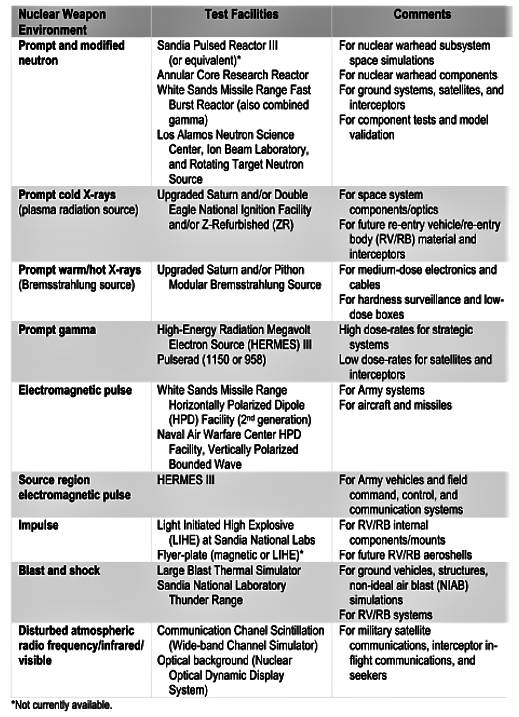
\includegraphics[width=\linewidth]{Figures/Chapter1/NWE.png}
	\label{tab:NWECap}
\end{table}

\ Previous work has shown that there is a capability gap to reproduce nuclear weapon effects (NWE) of interest to national security applications\cite{JointDefenseScienceBoard/ThreatReductionAdvisoryComitteeTaskForce2010, Bevins}. 
A key consideration for testing is the neutron energy spectrum in comparison with the environment that a nuclear weapon would see or produce. 
A particular spectrum of interest is the combination of a thermonuclear (TN) and prompt fission neutron spectrum (PFNS) as the present testing does not address this region to a large extent. 
The vast majority of testing facilities are focused on the Watt-fission spectrum, while a few are capable of producing the 14.1 MeV TN component from the deuterium-tritium (DT) fusion process\cite{Bridgman}. 
The current prompt neutron facilities available are not well suited for the TN+PFNS application testing because of the lack of high energy neutrons, or there is not a large enough flux of neutrons on target. 
Several examples of testing facilities for prompt neutrons outlined in Table \ref{tab:NWECap} are the Sandia Pulsed Reactor III (SPR), Sandia Annual Core Research Reactor (ACCR), White Sands Missile Range (WSMR) Fast Burst Reactor (FBR), the Los Alamos National Laboratory (LANL) Rotating Target Neutron Source (RTNS), and the LANL Weapons Neutron Research facility (WNR). 
The differential spectral profile of these sources compared to a notional TN+PFNS is shown in Figure \ref{fig:CompSource}. 

\begin{figure}[ht]
	\centering
	\includegraphics[width=\linewidth]{Figures/Chapter1/SourceComparison.png}
	\caption[Comparison of selected neutron sources to notional TN+PFNS]{Comparison of selected neutron sources to notional TN+PFNS {\cite{Bevins}}}
    \label{fig:CompSource}
\end{figure}

\ Each of the available neutron sources has an important purpose for national security applications; however, they cannot meet the energy spectrum of every nuclear testing requirement. 
In comparison with the TN+PFNS, nearly all of the neutron sources are heavily weighted to lower energies and do not contain enough high energy neutrons for the TN component. 
The RTNS has a high energy component, but the magnitude of the flux is substantially lower than required for some applications. 
The temporal aspect of the neutron flux also does not generally match to a nuclear weapon spectrum. 
Additionally, these large facilities often go underfunded or are shutdown. 
For example, the SPR-III was decommisioned in late 2006. % Moved this to SPR-III. It is hard to track where these systems are because they get started up again, and then shut down again... It operated after this at Berkeley for some time I believe.
Gathering accurate experimental results requires a neutron flux spectrum equivalent to that of a true nuclear event, which creates a need for a neutron source capable of emulating the environment. 
Therefore, development of a TN+PFNS source would enable production of the correct fission product inventory in surrogate debris and thereby enhance the ability of the TNF community to perform the attribution mission. 

% Move next two sentences to background?
%This is because nuclear fission yields as a function of energy is an area of nuclear physics for which little data exists and models perform poorly. Additionally, this is an area that was not captured well in the nuclear testing era due to a different geo-political environment where terrorist use of a nuclear weapon was a much smaller concern.  

\section{Background}

\ Many approaches can be used to create nuclear weapon relevant neutron spectra in the absence of full-scale nuclear weapons testing. Some mechanisms are more applicable within different communities in nuclear sciences. Four main possible ways that the neutron environments are approximated for synthetic fission product debris production are sample doping, direct production using fission converters, surrogate methods, and spectral modification of existing sources\cite{Bevins}. In the context of neutron effects on electronics, the key approaches utilized are using existing source, computational models, and surrogate charged particle reactions. Each of these methods are limited in representing the neutron environment experienced in a nuclear weapon. 

\ The sample doping technique irradiates with sources to build up a sample that is subject to a desired energy dependent fluence for the application, but the process is time and/or manpower intensive and the neutron fluence is not prompt requiring several corrections to the sample. 
A somewhat common TNF application using sample doping is the production of glass surrogate fallout debris for use in exercises or training\cite{Carney2014b}. 
The glassy matrix is created to emulate the solidified fission debris and entrained environment that is swept up in the stem of a nuclear explosion. 
The glass is doped with uranium and irradiated under various neutron environments depending on the requirements; however, the irradiation often done with a thermal neutron reactor. 
Additionally, the sample doping technique can be approached by irradiating different samples at different facilities. A final sample which has the ``correct'' fission product ratios can be created by selectively pulling mass chains from  the irradiated samples. 
This sample doping technique creates a fission product debris sample; however, the spectral and temporal nature of the sample is not equivalent to what would be produced in a real nuclear explosion.
% This is missing the main approach used by LLNL to create samples by irradiating samples at different facilities, selectively pulling mass chains from those samples, and then combining them into the a new sample in the correct ratios. This falls under the same category right? Thats what I think. 

\ Direct conversion utilizes nuclear reactions to create a shaped neutron flux, which can be done via charged particle interactions or through fusion sources with a fission converter. 
It has been shown that direct production is ``impractical, complex, and unlikely to be implemented for safety or technological limitations"\cite{Bevins}. 

\ Surrogate methods rely on the formation of an equivalent compound nucleus through an alternative reaction mechanism\cite{DIETRICH2007237,Scielzo2012}. 
Surrogate methods are popular in studies where forming the product nucleus through the desired reaction is difficult or the energy cannot be fine-tuned. 
An example of this is neutron induced fission on U-235. 
A possible surrogate for U-235 neutron induced fission reaction, (n,f), is Th-232 ($\alpha$,f), where the U-236 compound nucleus is formed. The surrogate reaction is useful for studying the fission products from 14 MeV neutron induced fission. The fission process is a function of the compound nucleus and independent of formation; however, the nucleus retains momentum, energy, spin, and parity \cite{Narek1}. A 25.6 MeV $\alpha$ particle provides the same excited state U-236 as a 14 MeV neutron in this example \cite{Narek1}. The surrogate approach has seen success; however, the nuclear data supporting the reactions is not as well understood\cite{RevModPhys.84.353,Narek1}. 
Additionally, there are some assumptions on the compound nuclear equilibration and spin-parity state which can impact the decay channels of the studied reactions \cite{DIETRICH2007237}.

\ Another commonly used surrogate method is to utilize charged particles for neutron damage in radiation effects on electronics. 
Ion beams can be used as a surrogate for neutrons by comparing the relative displacements per atom caused by the charged particle compared to a neutron\cite{Galy2018}. 
A major benefit of using ion beams is that the energy can be finely tuned both in energy and deposition location, whereas neutrons are not as easily controlled. 
A disadvantage of using charged particles is that a large portion of the energy deposition as it travels through materials is based on electronic stopping power, while the neutral neutrons have negligible interactions. 
The Qualification Alternatives to the Sandia Pulsed Reactor (QASPR) program is the most significant venture into the use of surrogate ions to perform neutron effects component level testing as a replacement alternative for the SPR\cite{JointDefenseScienceBoard/ThreatReductionAdvisoryComitteeTaskForce2010}. 
QASPR combines operational irradiation facilities with modeling to predict neutron effects. 
While there have been substantial improvements to increasing the verification and validation of simulated data to experimental outcomes, the validation for the experimental data benchmarked to neutron experimental data is lacking in many cases\cite{Bouchard}.

\ The final approach that could be used is spectral modification,  a method of altering a neutron spectrum through nuclear interactions to generate an energy spectrum of interest. 
Fundamentally, spectral modification is the goal of water moderated nuclear reactors to increase efficiency and allow the use of low enriched fuel. 

\ Spectral modification is also performed in beam shaping assemblies used for boron neutron capture therapy (BCNT) where a neutrons are used to treat tumors through neutron capture reactions in boron. 
A somewhat optimized objective neutron spectrum focused on the epithermal region is published by the International Atomic Energy Agency (IAEA) \cite{Kasesaz2016}. 
BCNT has been explored with a wide variety of sources including accelerators and deuterium-deuterium (DD) fusion. 
A beam shaping assembly can be designed to moderate a source neutron flux to appropriate thermal, eipthermal, and fast spectrum for BCNT\cite{Ardana2017}. 
The build up of a design is produced primarily through moderation, reflection, and collimation of neutrons to the patient \cite{Zaidi2018}. 
However, the approach to designing a beam shaping assembly lends itself to inefficiencies from an energy and population perspective.  % How so?

A novel approach spectral modification approach was developed by the University of California-Berkeley and Lawrence Livermore National Laboratory (LLNL) for the development of an energy tuning assembly (ETA) to modify the National Ignition Facility (NIF) source to produce a TN+PFNS\cite{Bevins}. 
To perform the spectral modification, the Coeus metaheuristic optimization software package was developed to avoid manpower intensive iterative studies and enable the rapid design of future ETAs to convert a facility's characteristic source spectrum to any arbitrary objective spectrum, within the constraints of physics\cite{Coeus}. 
%For their study, the design constraints included the mechanical envelope at the NIF, a 75 kg mass limit, material limitations, and efficiency requirements. 
%The nearly-globally optimum solution produced by Coeus was modified slightly to reduce cost and improve manufacturability. 
% I'd eliminate
Gnowee, the Coeus opimization engine, was developed for ``rapid convergence to nearly globally optimum solutions" of this class of engineering problems\cite{Bevins2018}. 
It is important to note that the Gnowee and Coeus codes have applicability over a wide range of engineering problems, not just for the production of a TN+PFNS.  

The result of the ETA design produced an acceptable representation of the TN+PFNS with the associated fission product distribution. 
The ETA design has been built and preliminary validation tests were conducted at the Lawrence Berkeley National Laboratory’s 88-Inch Cyclotron \cite{Bevins, Stickney}. 
The preliminary validation utilized 33 MeV deuterium breakup on tantalum as a neutron source and investigated the ability to model the ETA performance \cite{Stickney}.
Integral validation is planned in fiscal year (FY) 2019, and a development shot to enhance ETA performance is planned in FY2020. 

% I'd delete the following section.  Maybe move the second sentence to the theory section where you discuss covariance.
%The future work relevant to the original ETA design following the 88-Inch Cyclotron experiment includes updates to fully propagate nuclear data uncertainties. 
%Two options for quantifying nuclear data uncertainty are Mercury with tools developed at LLNL and the SAMPLER module in SCALE developed by Oak Ridge National Laboratory (ORNL). 
%Two shots have been awarded at the NIF for ETA experiments.
 
\section{Problem} \label{problem}
%While the previous work was pretty awesome, it had several deficiencies that need addressed.  % You'll probably want to modify, but a transition stement like this would help
The previous work made great progress; however, there are several deficiencies that need to be addressed. The broad research objective for this work is \textit{Can an accurate neutron energy distribution expected from a "typical" thermonuclear or boosted nuclear weapon detonation be produced using spectral modification at the NIF?}. This research effort aims to address three main problem areas for ETA and spectral shaping of neutron sources for simulating nuclear weapon environments that were raised by previous work. Each are detailed below, organized by the experiment supported), along with accompanying research objectives. The enhanced ETA is referred to as "A THErmonuclear and prompt fission Neutron spectrum energy tuning Assembly" (ATHENA) for differentiation from the original ETA.

% I redid these so the numbered bullets read as a problem statements, and the bullets read as objectives
\begin{enumerate}
	\item FY 2019 NIF shot (ETA): Systematic uncertainty is not fully addressed in the previous ETA calculations
	\begin{itemize}
		\item Quantify the impact of nuclear data covariances of the simulated results for the neutron energy spectrum, foil activation rates, and fission product production rates
		\item Design a foil activation diagnostic pack to provide better resolution in the epi-thermal neutron energy range
		\item Prioritize and estimate production of fission products for radio-chemical analysis using recently published data
	\end{itemize} 
	
	\item FY 2020 NIF shot (ATHENA): The current ETA efficiency is too low for use as a production NTF and NWE source %you should introduce the NWE term somewhere above
		\begin{itemize}
			\item Develop a more representative neutron spectrum
			\item Update facility constraints to reflect recent NIF upgrades %TANDEM
			\item Develop a new ETA design to increase the ETA efficiency to produce $\sim 10^{12}$ fissions
		\end{itemize}		 
	
	\item FY 2020 NIF shot (ATHENA): The ETA at NIF was not evaluated for use as a `short pulse' neutron source (SPNS)
		\begin{itemize}
			\item Model the neutron timing profile and expected flux
			\item Incorporate the ability to measure the neutron time profile into the FY 2020 ETA design
		\end{itemize}		

\end{enumerate} 


\section{Questions and Hypothesis}
The research questions and hypotheses associated with the problems outlined in Section \ref{problem} are detailed below.  
They are organized by the problem and capability that they support.

\begin{enumerate}
	\item 2019 ETA Fission Product Experiment
	
	\begin{itemize}
		\item \textbf{What is the impact of nuclear data covariance on the simulated results?} It is expected that including nuclear data uncertainty will increase the relative error by approximately 1\% for integrated and well understood reactions and may extend over 10\% for less  studied reactions thereby dominating Monte Carlo statistical uncertainty. 
		
		\item \textbf{Does the activation foil pack have sufficient coverage of the neutron spectrum to be used for unfolding?} It is expected the current design is not sufficent to robustly unfold the neutron spectrum should the model deviate from experimental results. The nuclear data covariance error will be used in lieu of radiation counting statistics to determine the activities associated with each foil. The unfolded results will indicate if the foil diagnostic pack is acceptable to unfold the ETA generated neutron spectrum.
		%, and the incident flux on the highly enriched uranium (HEU) foil is near the objective spectrum.....This can be done just by modeling the result!  You may also want to include a method to test the sensitivity of the unfold on guess spectrum - i.e. have a method to perturb the spectrum to use as the input a priori.  
		
	\end{itemize}
    \item 2020 ATHENA Surrogate Debris Experiment %I think we can really push towards this by then
    \begin{itemize}
    	\item \textbf{Can the ETA efficiency be increased to achieve $\mathbf{10^{11} - 10^{12}}$ fissions?} This will be a factor of 100 to 1000 over the original ETA design.  The gain will be possible due to NIF source development, changes to the design envelop, updated TN+PFNS objective spectrum, and changes to the optimization objectives. 
    	
    	\item \textbf{How well does the enhanced ETA perform to match the objective neutron environment?} The chi-square statistic will be used similarly to the goodness of fit criteria for the original ETA design. % The optimization used a flux weighted relative least squares fit - are you planning to use the chi sqaured? Also, there is not a hypothesis here...I'd probably delete? 
    \end{itemize}
	\item 2020 ATHENA SPNS Experiment
	\begin{itemize}
		\item \textbf{Can an ETA-SPNS be useful as a capability for testing of prompt neutron environments?} The original ETA design has a pulse length on the foils of approximately 1 ms for neutrons in the range of XX to YY MeV. It is anticipated that this can be optimized with Coeus and assessed against an objective spectrum and fluence. % I'd delete or incorporate into the first sentence: Additionally, the majority of the neutrons arriving on the foils is within approximately 100 shakes (100 $\mu s$) from the start of the neutron pulse on target. 
			
	\end{itemize}
\end{enumerate}

\section{Assumptions and Limitations}

An omnipresent limitation in many studies of science and engineering is the quality and quantity of available data for applications. 
Nuclear engineering commonly draws from published works containing the relevant nuclear data and the uncertainties behind them. 
The results presented are limited by the currently accepted understanding of nuclear physics phenomena and by the limitations of published data that is consistently being improved upon by the nuclear science community. 

The second limitation, which is done so for convenience and publishing ability, is that the nuclear weapon environments are presented at an unclassified level. 
All information used to develop the neutron flux and profile is available in open literature or derived from unclassified information to produce a representative environment. 
The accuracy of the representative neutron environment compared to a specific real-world nuclear weapon scenario was not analyzed and will not be presented. 
The scope of this work aims to provide a position where, if desired, one could easily go from the unclassified spectrum to one that fully meets a requirement. 

An assumption for this work is the choice of the NIF as the neutron source. 
Other sources may be present that would also perform the role, but NIF has unique benefits such as the prompt nature of the neutron yield and the fast neutrons arising from DT fusion. 
Although the NIF has been in operation since approximately 2010, there is a potential insertion of systematic error based on the source characterization and variability in the source output. 

Nuclear weapons can be categorized into three general classes: fission, boosted and TN\cite{Bridgman,Mctl}. 
It has been shown that the majority of the present capability to produce synthetic debris is most focused on the fission devices\cite{Bevins}. 
The TN+PFNS was chosen in previous work because it is an area that lacks substantial source development. 
It is important to note that there is not just one spectrum that can classify the TN+PFNS. 
The TN portion of the weapon spectrum is assumed to be pure DT fusion \cite{Mctl}. 
The impact of weapon design, which can vary substantially and play a large role in the resultant neutron energy spectrum, is not evaluated in this work. 

Some physical phenomena present in a true nuclear event are not taken into consideration for this analysis. 
First, the temperatures seen in nuclear weapons are on the order of $10^{7}$ K, which is not feasible for the experiment\cite{Glasstone1977}. 
Second, the time dependency of the internal neutron flux as the weapon is configured is not taken into account. 
Additionally, there will be large changes to the flux from initiation to burnout, and this work looks at a time and volume average result. 
Third, the synthetic weapon debris is created without induced fractionation. 
It is feasible to perform some level of fractionation; however, the levels of refractories and volatiles will not be altered in this work. 

\section{Approach}

The spectral shaping problem is defined by the objectives and constraints. 
For this research, the problem objectives are the ETA spectrum for fission product generation and ATHENA spectrum for enhanced fission product generation and SPNS. 
The problem constraints are based on the NIF source term and mechanical envelope. 
The input objectives and constraints are utilized in Coeus to produce a nearly-globally optimum solution for an ETA. 
The work performed previously has a completed design for the original ETA that will be used for all analysis of the expected experimental performance. 

Coeus is used as an optimization tool to develop ATHENA\cite{Bevins2018}. The constraints for the problem are governed by the NIF source which is modeled as the polar direct drive exploding pusher (PDXP), stay-out angle defined by the incident lasers to drive the fusion, and the constrains of the NIF Target and Diagnostic Manipulator (TANDM). The objective spectrum for ATHENA is an improved TN+PFNS with the goals of increasing the number of fissions in the HEU sample and better representing the neutron environment. The ATHENA objective spectrum is also appropriate for neutron effects on electronics testing for high altitude burst or space environments. The neutron energy distribution is modified by the atmosphere; however, negligible attenuation occurs in a near vacuum.  

\ The point designs are modeled with MCNP and SCALE version 6.2 to perform neutron radiation transport. 
MCNP is used for continuous energy solution, while SCALE is  used for group-wise covariance analysis. 
MCNP versions 5 and 6 are both used depending on compatibility with surface source read (SSR) files generated by the NIF and LLNL. 
Utilizing two different radiation transport models also increases the degree of confidence in the results. 
The radiation transport simulations provide results for the reaction rates for foil activation, neutron energy spectra, and temporal aspect of the neutron flux. 

\ A General Description of Fission Observables (GEF) is utilized for developing the expected fission product yields. 
GEF is a Monte Carlo and theory based approach that incorporates experimental data to determine fission observables, such as fission products \cite{Schmidt2016}. 
Empirical methods for determining fission product distributions also exist. 
A formulation of this fit by S. Nagy would be beneficial for comparison to GEF\cite{Nagy1978}. 
These empirical methods often include simplifications, such as ignoring neutron multiplicity, to create a simpler equation and more direct tie to existing data - both a benefit and limitation of this approach.  

\ A foil pack designed to be placed in the ETA experimental cavity will be created to be able to successfully unfold the incident neutron spectra from the activation foils. 
The activation foils are selected with many important factors including the confidence in the nuclear data and energy range that the foils are activated. 
The modeled foil activities are used with the underlying nuclear data to unfold the neutron spectrum using Pacific Northwest National Laboratory (PNNL) STAYSL. 
STAYSL relies on least-squares spectral adjustment based on the chi-squared of the measured activities to determine the incident neutron flux \cite{Greenwood2016}. 
The nuclear data-covariance uncertainty is used as the activation uncertainty in the unfolding, which will provide a higher level of confidence in the spectral agreement. 
The true activation uncertainty will almost certainly be below that of the nuclear data covariance sampled values. 


